\section{Milestone}
This section outlines the key milestones for the successful completion of the project, along with their respective timelines. The milestones are divided into distinct phases to ensure clarity and manageability throughout the project lifecycle.

\subsection{Project Milestones and Timeline}
The major milestones for the project are as follows:
\begin{enumerate}
    \item \textbf{Data Collection and Preparation (Week 1-4):}
    \begin{itemize}
        \item Collect the dataset of crop disease images.
        \item Perform data cleaning, augmentation, and preprocessing to ensure quality and consistency.
    \end{itemize}
    
    \item \textbf{Model Development and Training (Week 5-8):}
    \begin{itemize}
        \item Explore and implement machine learning and deep learning models.
        \item Train the models using the prepared dataset and tune hyperparameters.
    \end{itemize}
    
    \item \textbf{Model Evaluation and Optimization (Week 9-10):}
    \begin{itemize}
        \item Evaluate the models using defined metrics like accuracy, precision, and F1 score.
        \item Optimize the model to improve performance and handle class imbalances.
    \end{itemize}
    
    \item \textbf{Application Development (Week 11-12):}
    \begin{itemize}
        \item Develop a user-friendly application or interface for disease prediction.
        \item Integrate the trained model with the application for real-time predictions.
    \end{itemize}
    
    \item \textbf{Testing and Deployment (Week 13-14):}
    \begin{itemize}
        \item Test the application for accuracy, usability, and performance.
        \item Deploy the final system for end-user accessibility.
    \end{itemize}
\end{enumerate}

\subsection{Visualization of Timeline}
The timeline and schedule feasibility for the project phases are depicted in the Gantt chart below (Figure~\ref{fig:gantt-chart}).

\begin{figure}[H]
    \centering
    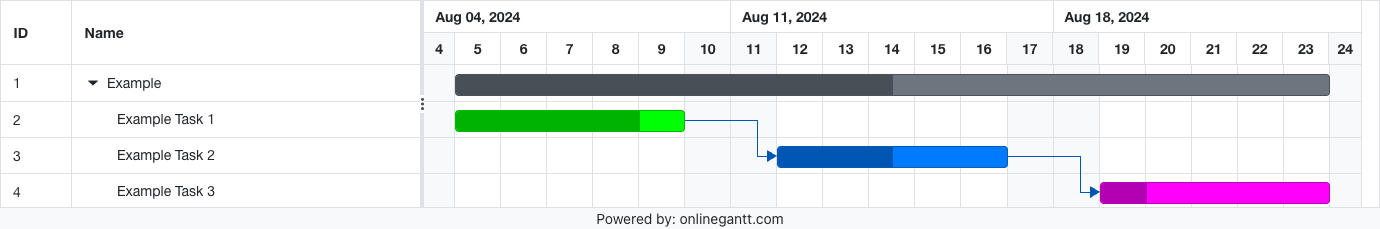
\includegraphics[width=1\linewidth]{Images/gantt.png}
    \caption{Sample Gantt Chart demonstrating schedule feasibility}
    \label{fig:gantt-chart}
\end{figure}
